\chapter{Qt Formen}
\begin{figure}[H]
	\begin{subfigure}{0.245\textwidth}
		\centering
		\begin{tikzpicture}[every node/.style={black, fill ,circle, inner sep = 1pt}]
		\node[label = {$V_0$}, rotate = 135] at (0,0) (V0) {};
		\node[label = {$V_1$}, rotate = -45] at (1,1) (V1) {};
		\node[label = {$V_2$}, rotate = 135] at (2,0) (V2) {};
		\node[label = {$V_3$}, rotate = -45] at (3,1) (V3) {};
		
		\draw (V0) -- (V1) (V2) -- (V3);
		\end{tikzpicture}
		\caption{\texttt{GL\_LINES}}
	\end{subfigure}
	%
	\begin{subfigure}{0.245\textwidth}
			\centering
		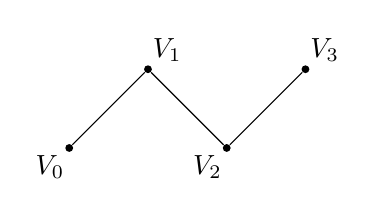
\begin{tikzpicture}[every node/.style={black, fill ,circle, inner sep = 1pt}]
		\node[label = {$V_0$}, rotate = 135] at (0,0) (V0) {};
		\node[label = {$V_1$}, rotate = -45] at (1,1) (V1) {};
		\node[label = {$V_2$}, rotate = 135] at (2,0) (V2) {};
		\node[label = {$V_3$}, rotate = -45] at (3,1) (V3) {};
		
		\draw (V0) -- (V1) -- (V2) -- (V3);
		\end{tikzpicture}
		\caption{\texttt{GL\_LINE\_STRIP}}
	\end{subfigure}
	%
	\begin{subfigure}{0.245\textwidth}
				\centering
		\begin{tikzpicture}[every node/.style={black, fill ,circle, inner sep = 1pt}]
		\node[label = {$V_0$}, rotate = 135] at (0,0) (V0) {};
		\node[label = {$V_1$}, rotate = -45] at (1,1) (V1) {};
		\node[label = {$V_2$}, rotate = 135] at (2,0) (V2) {};
		\node[label = {$V_3$}, rotate = -45] at (3,1) (V3) {};
		\end{tikzpicture}
		\caption{\texttt{GL\_POINTS}}
	\end{subfigure}
	%
	\begin{subfigure}{0.245\textwidth}
				\centering
		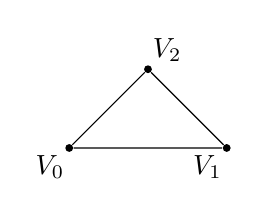
\begin{tikzpicture}[every node/.style={black, fill ,circle, inner sep = 1pt}]
		\node[label = {$V_0$}, rotate = 135] at (0,0) (V0) {};
		\node[label = {$V_2$}, rotate = -45] at (1,1) (V2) {};
		\node[label = {$V_1$}, rotate = 135] at (2,0) (V1) {};
		\draw (1,.4) node[fill=none, align=center, anchor=center] {\leftturn};
		\draw (V0) -- (V1) -- (V2) -- (V0);
		\end{tikzpicture}
		\caption{\texttt{GL\_TRIANGLE}}
	\end{subfigure}
	%
	\begin{subfigure}{.45\textwidth}
		\centering
		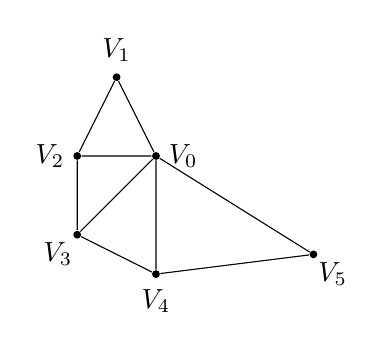
\begin{tikzpicture}[every node/.style={black, fill ,circle, inner sep = 1pt}]
			\node[label = {$V_0$}, rotate=-90] at (0,0) (V0) {};
			\node[label = {$V_1$}, rotate=0] at (-.5,1) (V1) {};
			\node[label = {$V_2$}, rotate=90] at (-1,0) (V2) {};
			\node[label = {$V_3$}, rotate=135] at (-1,-1) (V3) {};
			\node[label = {$V_4$}, rotate=180] at (0,-1.5) (V4) {};
			\node[label = {$V_5$}, rotate=-135] at (2,-1.25) (V5) {};
			
			\draw (V0) -- (V1) -- (V2)
			(V0) -- (V2) -- (V3)
			(V0) -- (V3) -- (V4)
			(V0) -- (V4) -- (V5) -- (V0);
		\end{tikzpicture}
		\caption{\texttt{GL\_TRIANGLE\_FAN}}
	\end{subfigure}
	%
	\begin{subfigure}{.45\textwidth}
			\centering
			\begin{tikzpicture}[every node/.style={black, fill ,circle, inner sep = 1pt}, xscale = 1.5]
			\node[label = {$V_0$}, rotate=180] at (0,0) (V0) {};
			\node[label = {$V_1$}, rotate=0] at (0,1) (V1) {};
			\node[label = {$V_2$}, rotate=180] at (1,0) (V2) {};
			\node[label = {$V_3$}, rotate=0] at (1,1) (V3) {};
			\node[label = {$V_4$}, rotate=180] at (2,0) (V4) {};
			\node[label = {$V_5$}, rotate=0] at (2,1) (V5) {};
			\node[label = {$V_6$}, rotate=180] at (3,0) (V6) {};
			\node[label = {$V_7$}, rotate=0] at (3,1) (V7) {};
			
			\draw (V0) -- (V1) -- (V2) -- (V0)
			(V1) -- (V2) -- (V3) -- (V1)
			(V2) -- (V3) -- (V4) -- (V2)
			(V3) -- (V4) -- (V5) -- (V3)
			(V4) -- (V5) -- (V6) -- (V4)
			(V5) -- (V6) -- (V7) -- (V5);
			
			\draw ($ 1/3*(V0)+1/3*(V1)+1/3*(V2)$) node[fill=none] {\rightturn};
			\draw ($ 1/3*(V1)+1/3*(V2)+1/3*(V3)$) node[fill=none] {\leftturn};
			\draw ($ 1/3*(V2)+1/3*(V3)+1/3*(V4)$) node[fill=none] {\rightturn};
			\draw ($ 1/3*(V3)+1/3*(V4)+1/3*(V5)$) node[fill=none] {\leftturn};
			\draw ($ 1/3*(V4)+1/3*(V5)+1/3*(V6)$) node[fill=none] {\rightturn};
			\draw ($ 1/3*(V5)+1/3*(V6)+1/3*(V7)$) node[fill=none] {\leftturn};
			\end{tikzpicture}
			\caption{\texttt{GL\_TRIANGLE\_STRIP}}
		\end{subfigure}
\end{figure}